%% Calibration Robustness of Photometric Star/Galaxy/Quasar Classifiers Under Magnitude Shift
%% IEEE conference format (IEEEtran). Compile on Overleaf: set the main document to this file
%% and press Recompile. Figures are read from ../figures/ (adjust \graphicspath if you move it).
\documentclass[conference]{IEEEtran}
\IEEEoverridecommandlockouts
\usepackage{cite}
\usepackage{amsmath,amssymb,amsfonts}
\usepackage{graphicx}
\usepackage{textcomp}
\usepackage[T1]{fontenc}
\usepackage[utf8]{inputenc}
\usepackage{xcolor}
\graphicspath{{figures/}{../figures/}}

\begin{document}

\title{Calibration Robustness of Photometric Star, Galaxy, and Quasar Classifiers Under Magnitude Shift}

\author{\IEEEauthorblockN{Joshua Anojulu}
\IEEEauthorblockA{Texas Academy of Mathematics and Science\\
University of North Texas, Denton, TX, USA\\
Email: joshanojulu@gmail.com}}

\maketitle

\begin{abstract}
Modern photometric surveys classify far more astronomical sources than can be confirmed spectroscopically, and increasingly rely on the \emph{probabilities} output by machine-learning classifiers to build clean samples and prioritize follow-up. Such probabilities are useful only if they are calibrated: an object assigned 90\% confidence should belong to the predicted class about 90\% of the time. While accuracy degradation toward faint magnitudes is well documented for photometric classification, the behavior of probability \emph{calibration} under this shift has not been studied for the star/galaxy/quasar problem. This work measures the calibration of four common classifiers on SDSS photometry and tracks how calibration changes with source magnitude. It further tests whether post-hoc recalibration (Platt scaling, isotonic regression, temperature scaling) fit on bright sources remains valid on faint ones. On a sample of 499{,}995 SDSS sources, the random-forest, gradient-boosted, and neural-network classifiers prove well calibrated (expected calibration error, ECE, of 0.003--0.005) and, contrary to the expectation set by their faint-end accuracy loss, remain so across the full magnitude range; calibration tracks model capability, with only the weaker logistic-regression model substantially miscalibrated (ECE 0.077). Post-hoc recalibration fit on bright sources transfers poorly to faint ones, most severely for Platt scaling (which inflates faint-bin ECE by roughly an order of magnitude), while temperature scaling is the most transfer-robust. For the well-calibrated models, a probability-thresholded quasar sample is as pure as its probabilities promise at every magnitude; the magnitude dependence appears in completeness, not purity. These results indicate that capable photometric classifiers can supply trustworthy selection probabilities across magnitude, that the principal risk lies in naive recalibration rather than in the base models, and that the dominant faint-end limitation is completeness. These findings are relevant to probabilistic source typing in LSST-era pipelines.
\end{abstract}

\begin{IEEEkeywords}
probability calibration, expected calibration error, photometric classification, distribution shift, post-hoc recalibration, sample selection, sky surveys.
\end{IEEEkeywords}

\section{Introduction}
Wide-field photometric surveys now catalog far more astronomical sources than can be observed spectroscopically. To assign source types---star, galaxy, or quasar---at this scale, surveys rely on supervised machine-learning classifiers trained on the comparatively small set of spectroscopically confirmed objects; one recent catalog applies such a model to more than one hundred million SDSS sources lacking spectra \cite{r10}. As the Vera C. Rubin Observatory's Legacy Survey of Space and Time (LSST) expands catalog volumes by orders of magnitude while spectroscopic follow-up remains scarce, probabilistic photometric classification is becoming the primary means of source typing. Supervised classification is now applied widely across astronomy, from time-domain stellar evolutionary-state typing \cite{r8} to survey-scale source classification.

Such classifiers report not only a predicted label but a probability for each class, and downstream analyses threshold or weight on these probabilities to assemble pure samples and to prioritize follow-up. A probability is trustworthy only if it is \emph{calibrated}: among all objects assigned a given confidence, the fraction that genuinely belong to the predicted class should equal that confidence. Calibration is distinct from accuracy---a classifier may be accurate yet systematically over- or under-confident---and contemporary classifiers are frequently miscalibrated, exhibiting characteristic over- or under-confidence that varies by model family \cite{r1,r2}.

Two largely independent lines of research bear on whether these probabilities can be trusted in the regime that matters most. Within astronomy, classifier accuracy is well known to degrade toward faint magnitudes, where labeled training data are sparse and unrepresentative, a consequence of sample-selection (Malmquist) bias; magnitude-resolved analyses of photometric star/galaxy/quasar classification confirm that faint sources are preferentially misclassified \cite{r9}. Within machine learning more broadly, probability calibration is well known to deteriorate under distribution shift, and post-hoc recalibration fit on in-distribution data has been shown to lose validity as the shift increases \cite{r5}. Calibration has begun to be examined in astronomical classification---reliability diagrams have been reported for gamma-ray source classifiers \cite{r6}, temperature scaling has been applied to supernova classification \cite{r7}, and calibration metrics have appeared for star/galaxy/quasar classifiers themselves \cite{r12}---yet how that calibration behaves under the very magnitude shift known to erode their accuracy, and whether a recalibration fit at bright magnitudes transfers to faint ones, has not been examined.

This work addresses that gap. Using SDSS photometry, this study (i) measures the calibration of four widely used classifiers on an independent test set, (ii) characterizes how calibration changes as a function of source magnitude, and (iii) determines whether a recalibration map fit on bright sources remains valid when applied to faint ones. The contribution is not a new classification algorithm but an empirical characterization of calibration robustness under magnitude shift for photometric source classification, together with its consequences for the probability-thresholded sample selection on which survey pipelines increasingly depend. The principal finding is one of robustness rather than degradation: the three higher-accuracy classifiers are well calibrated and remain so across magnitude, so calibration here is governed by model capability more than by the magnitude shift; the chief hazards are instead a poorly calibrated weak model and the tendency of bright-fit recalibration to degrade faint-end calibration, while the faint regime's principal cost falls on sample completeness rather than purity.

The remainder of this paper is organized as follows. Section~\ref{sec:methods} details the data, classifiers, calibration metrics, and the magnitude-shift protocol; Section~\ref{sec:results} reports results; and Section~\ref{sec:discussion} discusses limitations and implications for forthcoming surveys.

\section{Methods}\label{sec:methods}

\subsection{Data and Features}
Labeled data are drawn from the Sloan Digital Sky Survey (SDSS), using spectroscopic classifications as ground truth. Data Release 17 (DR17) is used for its well-characterized legacy spectroscopy and direct comparability with prior photometric-classification studies; the procedure applies unchanged to later releases. Spectroscopically confirmed objects with reliable redshifts (\texttt{zWarning}~$=0$) are selected from the clean \texttt{SpecObj} view and matched to their primary, clean photometric counterparts in \texttt{PhotoObjAll} via \texttt{bestObjID} (\texttt{clean}~$=1$, \texttt{mode}~$=1$), retaining only sources with class $\in \{$STAR, GALAXY, QSO$\}$.

Each source is described by its five dereddened model magnitudes ($u, g, r, i, z$) and the four adjacent colors ($u-g$, $g-r$, $r-i$, $i-z$). The spectroscopic redshift is deliberately excluded from the feature set: it is a near-perfect proxy for quasar identity and would dominate the model and trivialize the calibration analysis. The dereddened $r$-band magnitude is likewise withheld from the features and reserved to define the magnitude shift (Section~\ref{sec:shift}). The final sample comprises 499{,}995 objects---295{,}200 galaxies (59\%), 108{,}857 stars (22\%), and 95{,}938 quasars (19\%)---a class distribution set by SDSS spectroscopic targeting and, like the magnitude distribution, non-uniform (Section~\ref{sec:discussion}).

\subsection{Data Partitioning}
Sources are partitioned by object into three disjoint sets---a training set, a calibration set, and a test set (60/20/20, stratified by class to preserve class proportions; here 299{,}997 / 99{,}999 / 99{,}999). The classifier is fit on the training set; any post-hoc recalibration map (Section~\ref{sec:recal}) is fit \emph{exclusively} on the calibration set; and all reported calibration and accuracy metrics are computed on the held-out test set. This separation is essential: fitting a recalibration map on training-set scores---which are overfit and overconfident---or on the test set would invalidate the measurement. To quantify sampling variability, the entire fit--calibrate--evaluate protocol is repeated over 20 independent class-stratified splits, and every reported metric is given as the mean with a 95\% confidence interval across those splits.

\subsection{Classifiers}
Four classifiers spanning distinct model families and known calibration behaviors are compared: multinomial logistic regression, a random forest, a gradient-boosted decision-tree ensemble, and a multilayer perceptron (MLP). Each model's hyperparameters are selected by five-fold cross-validated grid search (minimizing negative log-likelihood) on the training split---the random forest over tree count and maximum depth, the gradient-boosted ensemble over learning rate and iteration count, the MLP over hidden-layer width and $L_2$ penalty, and logistic regression over its inverse regularization strength---and the selected configuration (here a depth-limited 300-tree forest and a 128--64 MLP) is held fixed across all repeated splits. Because selection uses a single reference split, the reported confidence intervals reflect split-to-split variability rather than hyperparameter-selection uncertainty. Each model emits a class-probability vector (via \texttt{predict\_proba} for the tree- and regression-based models and a softmax output layer for the MLP), and the predicted class is the argmax of that vector.

\subsection{Calibration Metrics}
Calibration is assessed graphically with reliability diagrams, which plot empirical accuracy against predicted confidence in bins of confidence; the identity line denotes perfect calibration, with deviations above (below) it indicating under- (over-) confidence. Because the task is three-class, top-label calibration is summarized---the confidence of the predicted class, $\max_k p_k$---and per-class one-vs-rest reliability diagrams (Fig.~\ref{fig:perclass}) and calibration errors are also reported.

Calibration is quantified by the Expected Calibration Error (ECE),
\begin{equation}
\mathrm{ECE} = \sum_{m=1}^{M} \frac{|B_m|}{N}\,\bigl|\,\mathrm{acc}(B_m) - \mathrm{conf}(B_m)\,\bigr|,
\end{equation}
the sample-weighted mean gap between accuracy and confidence across $M$ confidence bins, together with the Maximum Calibration Error (the largest such gap). Two proper scoring rules that jointly reward calibration and sharpness are also reported: the multiclass Brier score \cite{r4} (mean squared error between the predicted probability vector and the one-hot label) and the negative log-likelihood. Because ECE is sensitive to the binning scheme \cite{r3}, it is reported with both equal-width and equal-mass (quantile) bins and at two bin counts (15 and 10).

\subsection{Recalibration Methods}\label{sec:recal}
Three standard post-hoc recalibration methods, each fit on the calibration set, are evaluated against the uncalibrated baseline: Platt (sigmoid) scaling and isotonic regression, both applied one-vs-rest for the multiclass setting, and temperature scaling. Temperature scaling divides the logits by a single scalar $T>0$ before the softmax,
\begin{equation}
p_k = \mathrm{softmax}(z_k / T),
\end{equation}
with $T$ chosen to minimize the negative log-likelihood on the calibration set; because it does not alter the argmax, it leaves classification accuracy unchanged, a property used as a consistency check. Calibration metrics and temperature scaling are implemented directly; Platt (sigmoid) and isotonic recalibration use scikit-learn's \texttt{CalibratedClassifierCV} applied to a frozen, already-fitted base estimator so that the recalibration map is fit only on the calibration set.

\subsection{Magnitude-Shift Protocol}\label{sec:shift}
The central experiment tests whether calibration is preserved under the magnitude shift that characterizes real survey application. The test set is divided into five dereddened-$r$ magnitude bins (edges at 14, 17, 18, 19, 20, 22), and a binary bright/faint split is defined at $r=19$. Calibration metrics are computed within each magnitude bin for (i) the uncalibrated model, (ii) a recalibration map fit on a representative (all-magnitude) calibration set, and (iii) a recalibration map fit on bright sources only. Comparing (iii) across bins isolates the \emph{transfer gap}, the degree to which a recalibration learned on bright sources fails on faint ones, which is the quantity of primary interest. Because the SDSS spectroscopic sample is magnitude-limited and target-selected, the faint regime is not a representative faint population; this limitation, and its bearing on interpretation, is addressed in Section~\ref{sec:discussion}.

Because class composition itself varies strongly across the magnitude bins, classwise calibration error is also reported within each bin: for each class, the predicted probability of that class is compared, one-versus-rest, to the empirical frequency of that class. Unlike aggregate top-label ECE, this controls for the changing class mix, so a flat classwise trend would indicate that any magnitude robustness reflects calibration itself rather than the shifting class proportions.

\subsection{Decision-Relevant Selection Quality}
To translate calibration error into a concrete observational cost, the analysis also measures the quality of a probability-thresholded sample. Taking the quasar class as the science target, a candidate sample is formed from all test objects with $P(\mathrm{QSO}) \geq \tau$ (default $\tau=0.9$). For this sample the \emph{achieved purity} (the true fraction of quasars among the selected objects) and \emph{completeness} (the fraction of all true quasars recovered) are computed within each magnitude bin, and compared against the \emph{promised purity}, the mean predicted $P(\mathrm{QSO})$ of the selected objects, which for a perfectly calibrated model equals the achieved purity. The gap between promised and achieved purity is thus a direct, decision-relevant measure of miscalibration: the degree to which a probability-selected sample is less pure than its probabilities claim. This gap is evaluated by magnitude bin for the uncalibrated model and after representative- and bright-only recalibration. The principle that well-calibrated probabilities allow sample purity and completeness to be read directly from a threshold is established \cite{r11}; the contribution here is to trace its breakdown across magnitude and its recovery by recalibration.

\section{Results}\label{sec:results}

\subsection{Baseline Calibration}
On the held-out test set (99{,}999 objects), the random forest, gradient-boosted trees, and MLP reach comparable accuracy (0.92--0.93) and are all well calibrated, with ECE between 0.003 and 0.005 (Table~\ref{tab:baseline}; Fig.~\ref{fig:reliability}); 95\% confidence intervals over the 20 splits are narrow (ECE half-widths $\leq 0.001$), so these differences are statistically resolved. HistGB and the MLP are the best calibrated (ECE 0.003 and 0.004), the random forest close behind (0.005), and all three show small maximum calibration errors (0.045--0.062). Logistic regression is the outlier on both axes: it is the least accurate (0.81) and by far the least calibrated (ECE 0.077, MCE 0.161), reflecting the limited capacity of a linear model on this feature space. Calibration here therefore tracks model capability rather than being a uniform property of the task.

\begin{table}[t]
\caption{Accuracy and calibration on the held-out test set. Values are means over 20 stratified splits; 95\% confidence intervals are narrow (ECE half-widths $\leq 0.001$).}
\label{tab:baseline}
\centering
\renewcommand{\arraystretch}{1.2}
\begin{tabular}{lccccc}
\hline
\textbf{Model} & \textbf{Acc.} & \textbf{ECE} & \textbf{MCE} & \textbf{Brier} & \textbf{NLL}\\
\hline
Logistic regression & 0.810 & 0.077 & 0.161 & 0.311 & 0.553\\
Random forest       & 0.925 & 0.005 & 0.045 & 0.113 & 0.210\\
HistGB              & 0.924 & 0.003 & 0.056 & 0.114 & 0.211\\
MLP                 & 0.926 & 0.004 & 0.062 & 0.112 & 0.207\\
\hline
\end{tabular}
\end{table}

\begin{figure}[t]
\centering
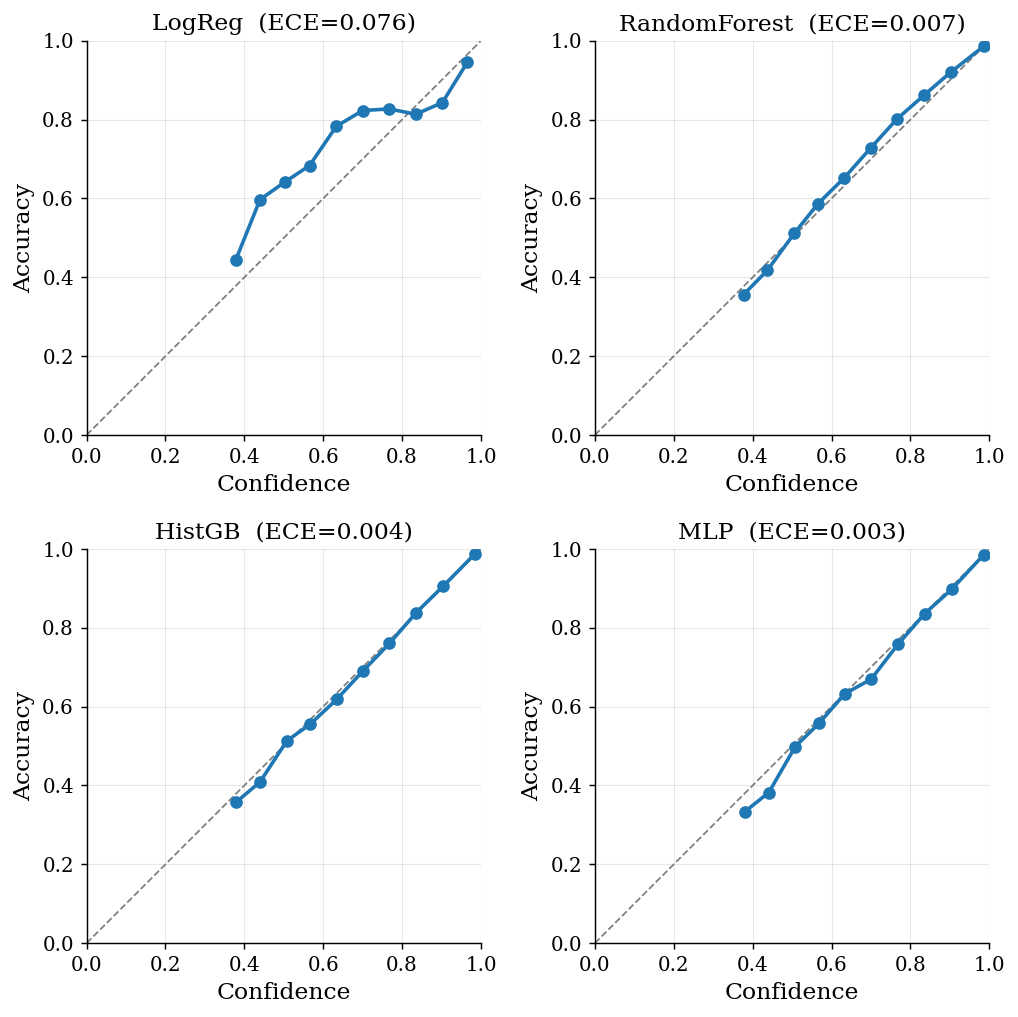
\includegraphics[width=\columnwidth]{fig1_reliability_baseline.png}
\caption{Reliability diagrams on the held-out test set. The three strong models track the diagonal closely (ECE 0.003 to 0.005); logistic regression is visibly miscalibrated.}
\label{fig:reliability}
\end{figure}

\begin{figure*}[t]
\centering
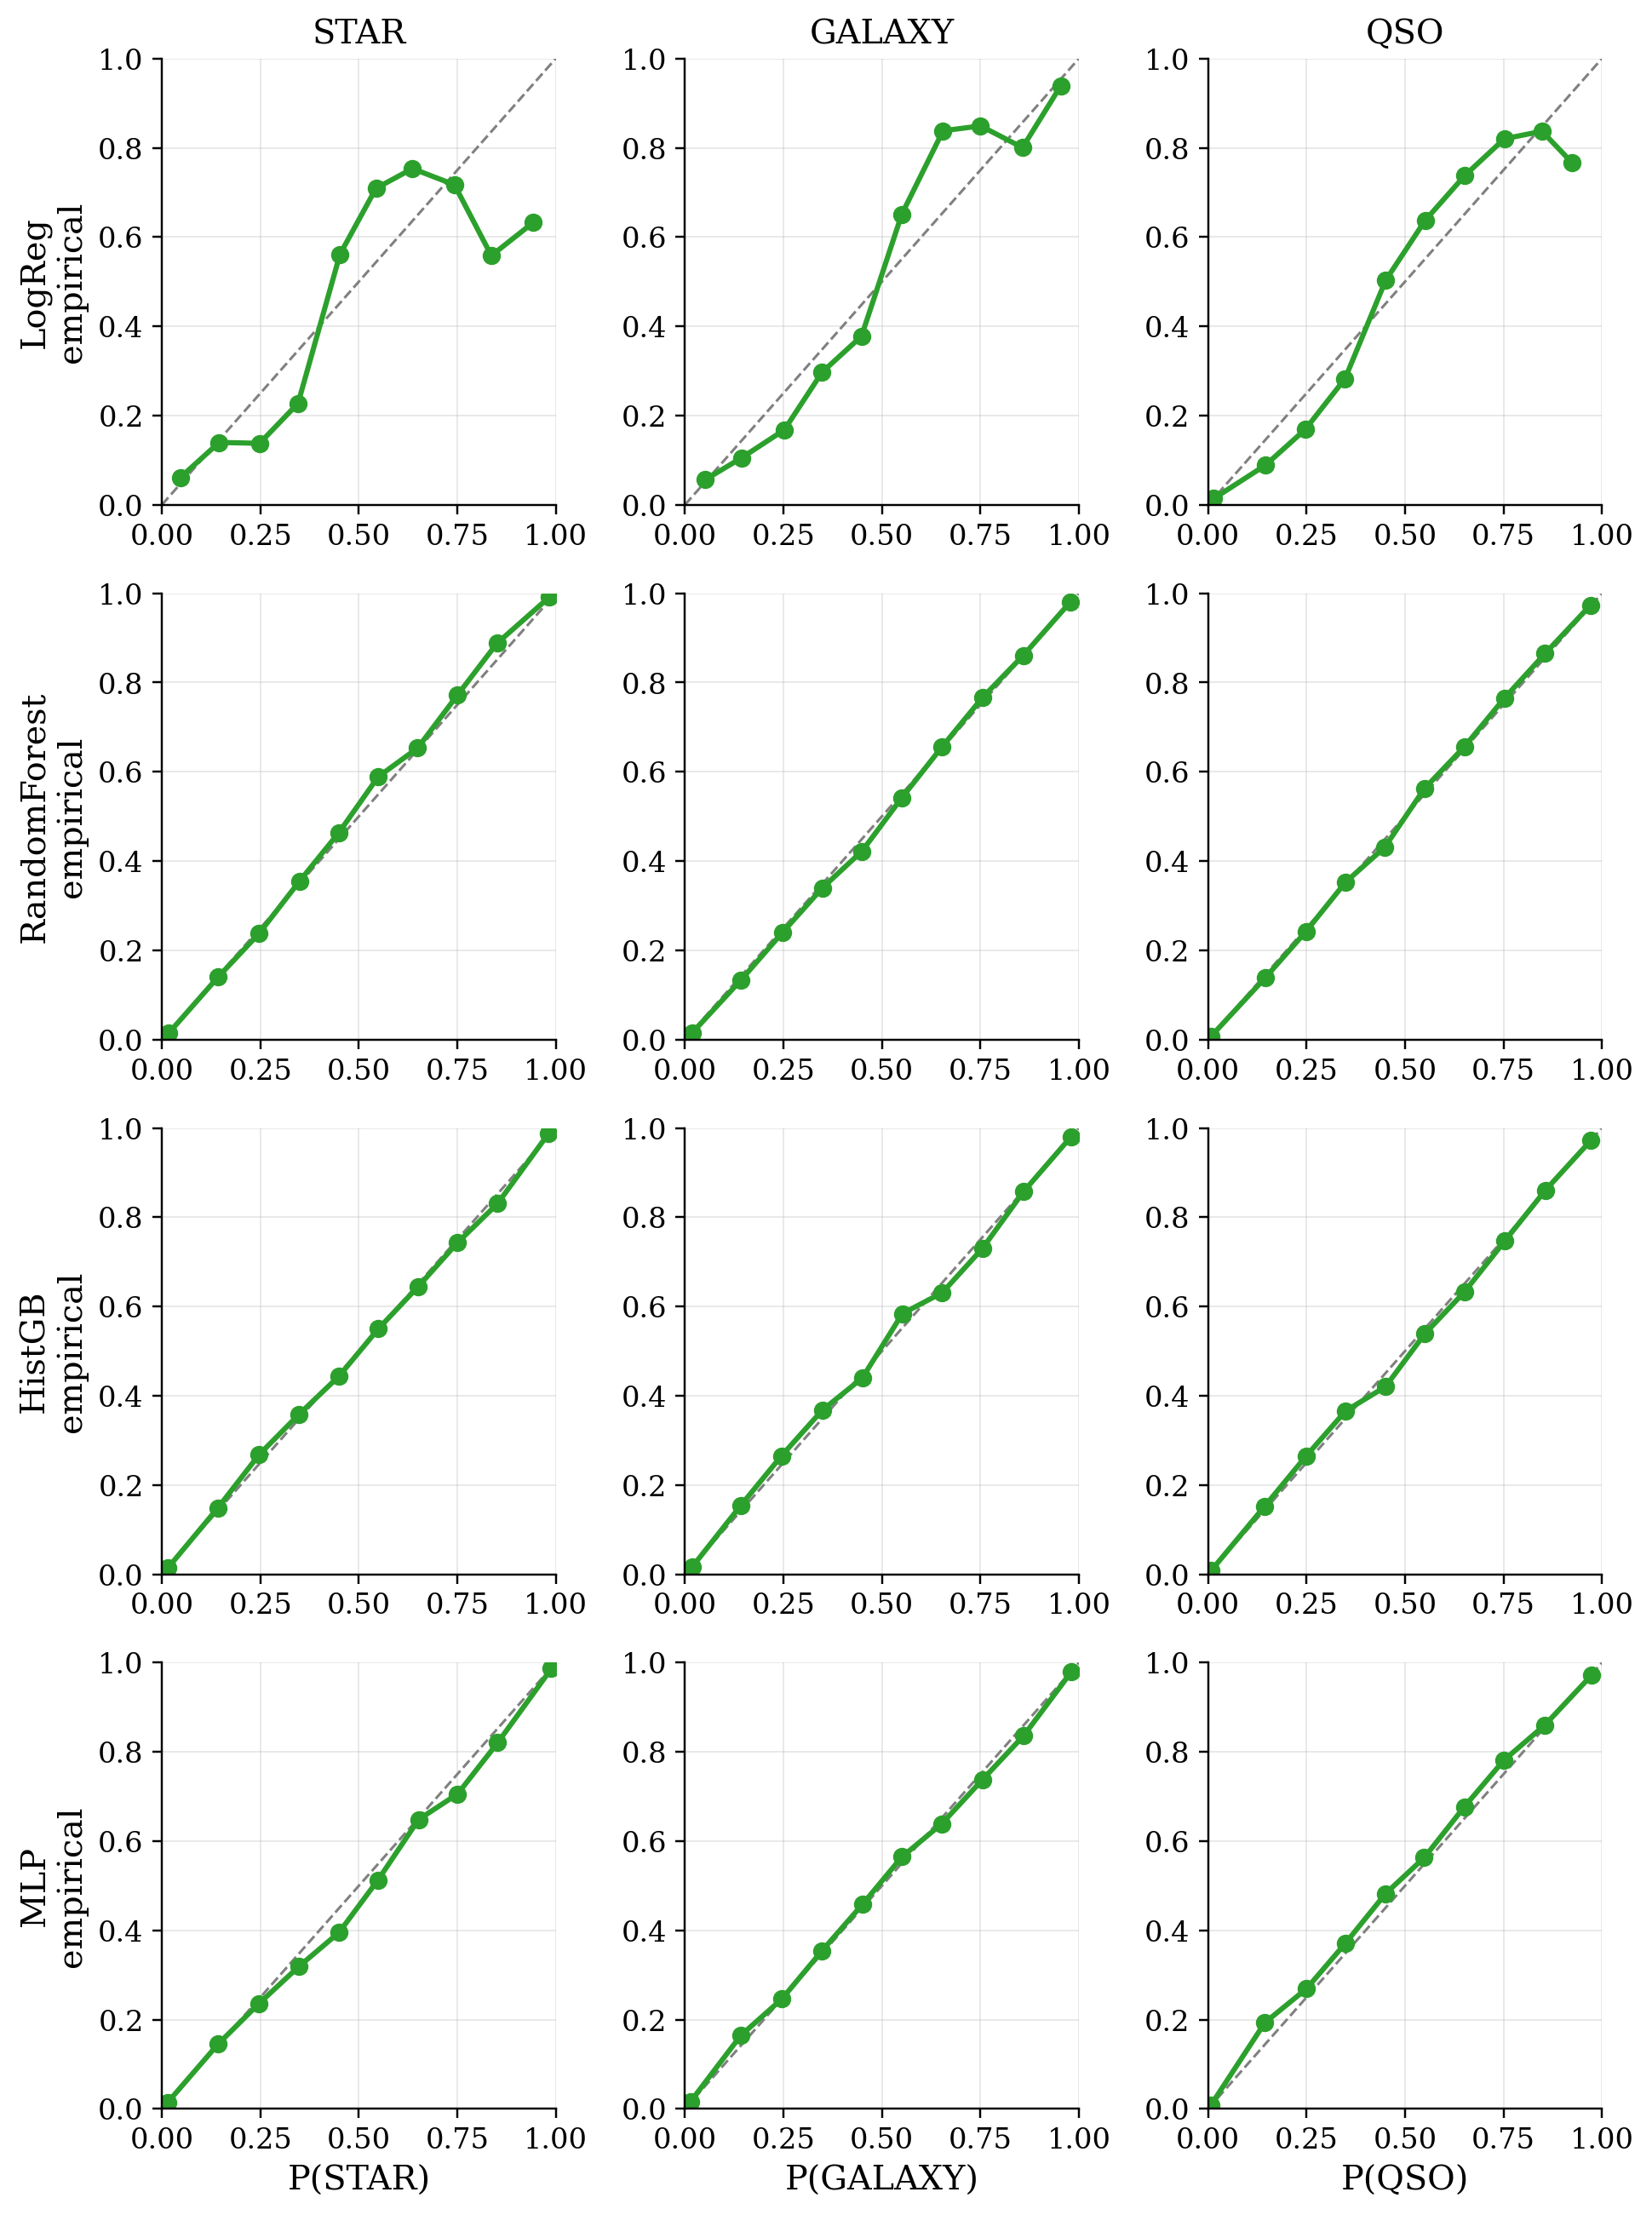
\includegraphics[width=0.82\textwidth]{fig1b_perclass_reliability.png}
\caption{Per-class one-vs-rest reliability diagrams (rows: models; columns: STAR, GALAXY, QSO). The three strong models hug the diagonal for every class; logistic regression deviates markedly.}
\label{fig:perclass}
\end{figure*}

\subsection{Calibration as a Function of Magnitude}
Figure~\ref{fig:ecemag} resolves calibration across five $r$-band magnitude bins. For the three strong models, top-label ECE is low and essentially flat from the bright to the faint end---random forest 0.006 (brightest) to 0.004 (faintest), peaking near 0.012 in between, HistGB ${\sim}0.003$--$0.006$ throughout, and MLP $0.003 \to 0.006$---with no systematic degradation toward faint sources. The expectation that calibration would erode under the magnitude shift is thus not borne out for capable models. Logistic regression again behaves differently: its ECE is highest in the brightest bin (0.17) and decreases toward the faint end (0.03), a trend opposite to the hypothesis and attributable in part to the changing class composition across magnitude (Section~\ref{sec:discussion}). Accuracy for the three strong models stays high across all bins; the dominant magnitude effect is therefore not on calibration but on the harder problem of recovering faint quasars, addressed in Section~\ref{sec:selection}.

To separate this from the strongly varying class mix across bins, classwise calibration error (one class versus the rest, which holds the class proportions out of the metric) is also computed per bin. For the random forest it is 0.005 in the brightest bin and 0.004 in the faintest (peaking near 0.009 in between), and the individual star, galaxy, and quasar terms each stay below 0.011 at every magnitude; HistGB and the MLP behave the same way. The flat classwise trend confirms that the magnitude robustness is intrinsic to the calibration rather than an artifact of the changing class proportions.

\begin{figure}[t]
\centering
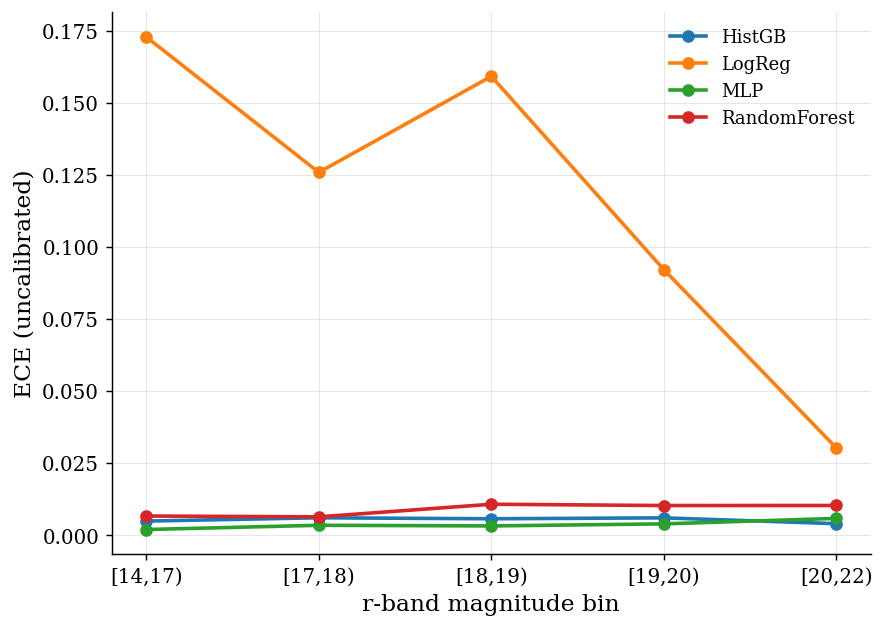
\includegraphics[width=\columnwidth]{fig2_ece_vs_magnitude.png}
\caption{Top-label ECE as a function of $r$-band magnitude. The three strong models stay flat and low across magnitude; logistic regression is high and decreasing.}
\label{fig:ecemag}
\end{figure}

\subsection{Recalibration Transfer}
Because the strong models are already well calibrated, recalibration offers little to gain and carries a real risk of harm. Platt scaling degrades calibration even when fit on a representative set (random-forest ECE rises from 0.005 to ${\approx}0.030$, MLP from 0.004 to ${\approx}0.031$), and fitting it on bright sources and applying it to the faintest bin is worse still---ECE reaches 0.063 for the random forest and 0.062 for the MLP. Isotonic regression shows a milder version of the same pattern. Temperature scaling is the most transfer-robust: a bright-fit temperature leaves faint-bin ECE near its uncalibrated value (random forest 0.017, MLP 0.007). The transfer result is therefore the inverse of the one anticipated---the danger is not that recalibration fails to fix a faint-end problem, but that recalibration, and bright-fit Platt scaling in particular, introduces one, with the severity depending strongly on the method (Fig.~\ref{fig:transfer}).

\begin{figure}[t]
\centering
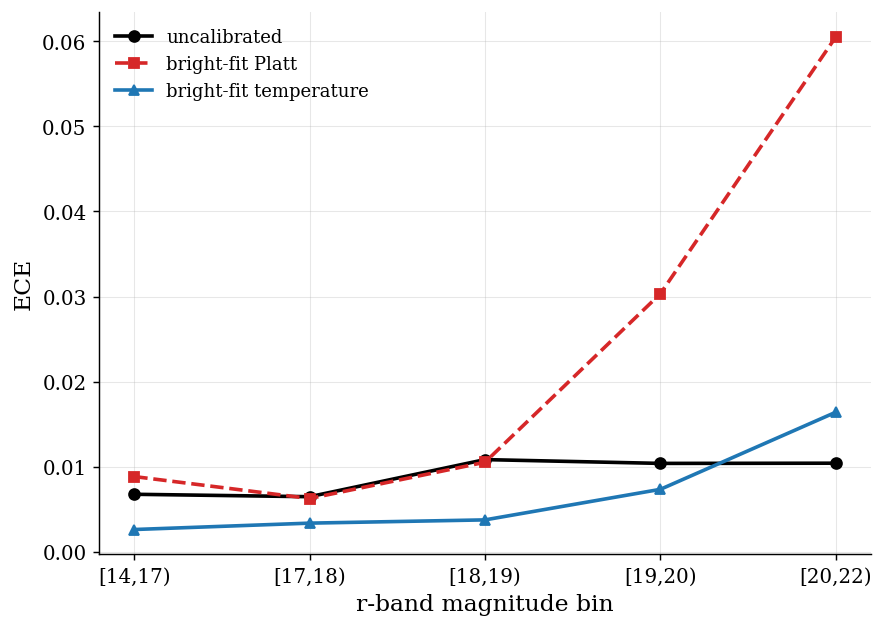
\includegraphics[width=\columnwidth]{fig3_recalibration_transfer.png}
\caption{Recalibration transfer for the random forest. A Platt map fit on bright sources degrades sharply at the faint end; temperature scaling transfers safely, staying near the uncalibrated baseline.}
\label{fig:transfer}
\end{figure}

\subsection{Decision-Relevant Selection Quality}\label{sec:selection}
Figure~\ref{fig:selection} recasts these calibration differences as the quality of a quasar sample selected at $P(\mathrm{QSO}) \geq 0.9$. For the well-calibrated models the achieved purity of the selected sample matches the purity its probabilities promise at every magnitude: the random forest's faint-bin sample ($r \in [20,22)$) is 96.3\% pure against a promised 96.3\%, and HistGB and the MLP agree with their promised purities to within about one percentage point likewise. The magnitude dependence appears instead in completeness, which falls toward faint sources, from ${\approx}0.77$ at $r \in [18,19)$ to ${\approx}0.52$ at $r \in [20,22)$ for the random forest, and similarly for the other strong models, because fewer faint quasars clear the 0.9 threshold. Logistic regression is the cautionary case: at the faint end it promises 92\% purity but delivers only 77\%, with completeness below 0.09, precisely the failure mode calibration is meant to prevent. For the strong models, recalibration changes these selections only marginally (a bright-fit temperature trades a fraction of a percentage point of purity for slightly higher completeness), consistent with the base probabilities already being trustworthy.

\begin{figure}[t]
\centering
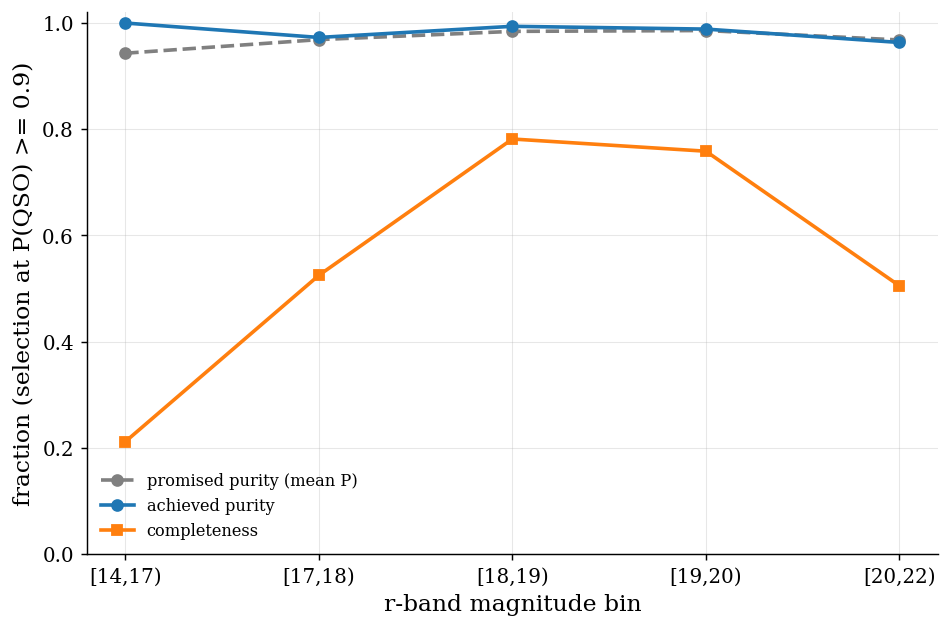
\includegraphics[width=\columnwidth]{fig4_selection_quality.png}
\caption{Quasar selection quality at $P(\mathrm{QSO}) \geq 0.9$ for the random forest. Achieved purity tracks the promised purity across magnitude; completeness falls toward faint sources.}
\label{fig:selection}
\end{figure}

\section{Discussion and Conclusion}\label{sec:discussion}
The central result is one of robustness. On SDSS photometry, the random-forest, gradient-boosted, and neural-network classifiers are well calibrated on the i.i.d.\ test set and remain so across the full magnitude range, so the calibration of these models is governed by model capability rather than by the magnitude shift that erodes faint-end accuracy. This echoes prior reports that a star/galaxy/quasar classifier can be well calibrated without explicit recalibration \cite{r12}, and it contrasts with the pronounced calibration-under-shift degradation documented for deep image classifiers \cite{r5}; the difference is plausibly that the photometric feature space and the tree, boosting, and MLP models used here do not become sharply overconfident as photometric errors grow.

Three qualifications temper this conclusion. First, calibration is not uniform across models: logistic regression is both less accurate and substantially miscalibrated, a reminder that calibration must be checked per model rather than assumed for the task. Second, the magnitude bins differ markedly in class composition---the bright bins contain very few quasars while the faint bins are quasar-dominated, a direct consequence of SDSS targeting quasars to faint magnitudes---so the magnitude axis is partly confounded with a changing class mix. The classwise calibration error reported in Section~\ref{sec:results}-B addresses this directly by holding the class proportions out of the metric; the apparent improvement of logistic-regression calibration toward faint sources should in any case be read in light of the shifting composition. Third, and relatedly, the spectroscopic sample is magnitude-limited and target-selected, so the faint sources studied here are not a representative faint population; calibration measured on this labeled sample may be optimistic relative to the full photometric faint population an LSST-era pipeline would face.

The practical implications are twofold. For sample selection, a capable, well-calibrated classifier delivers a probability-thresholded quasar sample whose purity matches its stated confidence at all magnitudes, so the probabilities can be trusted to set purity targets; the binding constraint at faint magnitudes is completeness, not contamination. For recalibration, the results counsel caution: because the base models are already calibrated, fitting a recalibration map on a convenient bright subset and applying it faint tends to introduce miscalibration rather than remove it, especially for Platt scaling, with temperature scaling the safest of the three methods.

In conclusion: (1) capable photometric star/galaxy/quasar classifiers are well calibrated, and that calibration is robust across magnitude, with miscalibration tracking model capability rather than the shift; (2) post-hoc recalibration transfers poorly across magnitude and can degrade calibration when fit on bright sources, temperature scaling least so; and (3) for probability-thresholded selection the faint-end cost falls on completeness while purity remains trustworthy. Future work should extend the analysis to a representative faint sample and to cross-survey transfer, where genuine covariate shift may stress calibration more than the within-survey magnitude shift studied here.

\begin{thebibliography}{99}
\bibitem{r1} C. Guo, G. Pleiss, Y. Sun, and K. Q. Weinberger, ``On calibration of modern neural networks,'' in \emph{Proc. 34th Int. Conf. Machine Learning (ICML)}, PMLR vol.~70, pp.~1321--1330, 2017. arXiv:1706.04599.
\bibitem{r2} A. Niculescu-Mizil and R. Caruana, ``Predicting good probabilities with supervised learning,'' in \emph{Proc. 22nd Int. Conf. Machine Learning (ICML)}, pp.~625--632, 2005.
\bibitem{r3} M. P. Naeini, G. F. Cooper, and M. Hauskrecht, ``Obtaining well calibrated probabilities using Bayesian binning,'' in \emph{Proc. 29th AAAI Conf. Artificial Intelligence}, pp.~2901--2907, 2015.
\bibitem{r4} G. W. Brier, ``Verification of forecasts expressed in terms of probability,'' \emph{Monthly Weather Review}, vol.~78, no.~1, pp.~1--3, 1950.
\bibitem{r5} Y. Ovadia et al., ``Can you trust your model's uncertainty? Evaluating predictive uncertainty under dataset shift,'' in \emph{Proc. NeurIPS}, 2019. arXiv:1906.02530.
\bibitem{r6} D. Malyshev and A. Bhat, ``Towards probabilistic multiclass classification of gamma-ray sources,'' arXiv:2209.10236, 2022.
\bibitem{r7} H. Qu, ``Towards precision photometric type Ia supernova cosmology with machine learning,'' Ph.D. dissertation, Univ. of Pennsylvania, 2024. arXiv:2406.04529.
\bibitem{r8} J. S. Kuszlewicz, S. Hekker, and K. J. Bell, ``Clumpiness: time-domain classification of red-giant evolutionary states,'' \emph{Mon. Not. R. Astron. Soc.}, vol.~497, no.~4, pp.~4843--4856, 2020. arXiv:2007.10921.
\bibitem{r9} F. Z. Zeraatgari et al., ``Machine learning-based photometric classification of galaxies, quasars, emission-line galaxies, and stars,'' \emph{Mon. Not. R. Astron. Soc.}, vol.~527, no.~3, pp.~4677--4689, 2024.
\bibitem{r10} A. O. Clarke, A. M. M. Scaife, R. Greenhalgh, and V. Griguta, ``Identifying galaxies, quasars, and stars with machine learning: A new catalogue of classifications for 111 million SDSS sources without spectra,'' \emph{Astron. Astrophys.}, vol.~639, p.~A84, 2020.
\bibitem{r11} P. C. Schneider et al., ``The eROSITA Final Equatorial-Depth Survey (eFEDS): the stellar counterparts of eROSITA sources identified by machine learning and Bayesian algorithms,'' \emph{Astron. Astrophys.}, vol.~656, 2022. arXiv:2106.14521.
\bibitem{r12} S. H. Bruun, J. Hjorth, and A. Agnello, ``Variability selection of astrophysical sources in PTF (VILLAIN) II: Supervised classification of variable sources,'' \emph{Astron. Astrophys.}, 2023. arXiv:2304.09905.
\end{thebibliography}

\end{document}
